\documentclass[tikz,border=4pt]{standalone}
% Shared style for every figure and for the deck: one accent, one
% highlight, thin lines, rounded nodes, nothing decorative.
\usepackage[T1]{fontenc}
\usepackage{lmodern}
\renewcommand{\familydefault}{\sfdefault}
\usepackage{tikz}
\usetikzlibrary{arrows.meta,positioning,calc,shapes.misc,fit,backgrounds,decorations.pathreplacing}
\definecolor{ink}{RGB}{40,40,40}
\definecolor{soft}{RGB}{150,150,150}
\definecolor{faint}{RGB}{225,225,225}
\definecolor{accent}{RGB}{0,95,115}
\definecolor{accentlight}{RGB}{214,232,236}
\definecolor{warn}{RGB}{196,84,40}
\definecolor{warnlight}{RGB}{247,226,216}
\tikzset{
  every picture/.style={color=ink, line width=0.5pt, font=\small},
  node distance=12mm and 18mm,
  box/.style={draw=ink, rounded corners=2pt, fill=white, inner sep=5pt, minimum height=7mm, align=center},
  maker/.style={box, minimum width=18mm},
  cat/.style={box, inner sep=3.5pt, minimum height=6mm},
  root/.style={box, fill=accentlight, draw=accent},
  bad/.style={box, fill=warnlight, draw=warn},
  ghost/.style={box, draw=soft, text=soft, dashed},
  flow/.style={-{Stealth[length=4pt,width=3.5pt]}, line width=0.5pt},
  sub/.style={-{Stealth[length=4pt,width=3.5pt]}, line width=0.5pt, color=soft},
  strong/.style={flow, color=accent, line width=0.8pt},
  wrong/.style={flow, color=warn},
  lbl/.style={font=\footnotesize, text=ink, inner sep=1.5pt, fill=white},
  note/.style={font=\footnotesize, text=soft, align=center},
  rate/.style={font=\footnotesize, text=accent, inner sep=1pt, fill=white},
}

\usepackage{amsmath}
\usepackage{pgfplots}
\pgfplotsset{compat=1.17}

\begin{document}
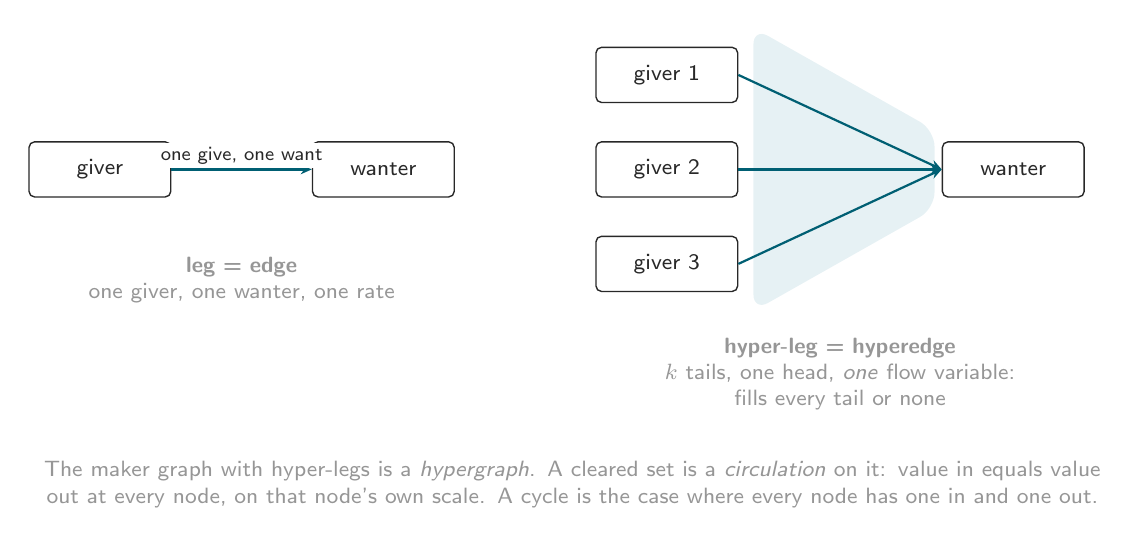
\begin{tikzpicture}[m/.style={box, font=\footnotesize, minimum width=18mm}]
  % An ordinary leg is an edge; a composed leg is a hyperedge with several
  % tails and one head and a single flow variable.
  \begin{scope}
    \node[m] (g) at (0,0) {giver};
    \node[m] (w) at (36mm,0) {wanter};
    \draw[strong] (g) -- node[lbl, above, font=\scriptsize] {one give, one want} (w);
    \node[note, text width=44mm] at (18mm,-14mm) {\textbf{leg = edge}\\ one giver, one wanter, one rate};
  \end{scope}
  \begin{scope}[xshift=72mm]
    \node[m] (g1) at (0,12mm) {giver 1};
    \node[m] (g2) at (0,0) {giver 2};
    \node[m] (g3) at (0,-12mm) {giver 3};
    \node[m] (w) at (44mm,0) {wanter};
    \begin{scope}[on background layer]
      \fill[accentlight, opacity=0.6, rounded corners=6pt] (11mm,18mm) -- (34mm,5mm) -- (34mm,-5mm) -- (11mm,-18mm) -- cycle;
    \end{scope}
    \foreach \g in {g1,g2,g3} { \draw[strong] (\g.east) -- (w.west); }
    \node[note, text width=60mm] at (22mm,-26mm) {\textbf{hyper-leg = hyperedge}\\ $k$ tails, one head, \emph{one} flow variable:\\ fills every tail or none};
  \end{scope}
  \node[note, text width=136mm] at (60mm,-40mm) {The maker graph with hyper-legs is a \emph{hypergraph}. A cleared set is a \emph{circulation} on it: value in equals value out at every node, on that node's own scale. A cycle is the case where every node has one in and one out.};
\end{tikzpicture}
\end{document}
